\section{Códigos QR}

\subsection{Captura y transmisión de imágenes}

Con el objetivo de mejorar la precisión en la estimación de posición del robot, incorporamos un sistema de captura de imágenes utilizando un microcontrolador ESP32-CAM equipado con una cámara $OV2640$. Esta solución reemplaza a sensores ultrasónicos usados en versiones anteriores de la familia Hermes, cuya precisión era escasa para aplicaciones de navegación detallada y además no representa un costo significativo para la gran oportunidad que se abre al usar el procesamiento de imágenes como método de localización y hasta en futuras implementaciones de navegación autónoma. \cite{dey2018hands}

Empleamos la ESP32-CAM, limitada en capacidad de procesamiento, solo para capturar imágenes y enviarlas vía comunicación inalámbrica utilizando el protocolo MQTT a un servidor central. Allí, una PC host ejecuta el procesamiento de imágenes en conjunto con la interfaz de usuario del sistema.

Para lograr una frecuencia aceptable de captura, optimizamos el sistema para alcanzar una resolución HD con una tasa de hasta 2 imágenes por segundo. Esta configuración permite realizar detecciones eficientes sin comprometer el desempeño general del sistema.

\subsection{Medición de distancia a códigos QR}

Utilizamos el reconocimiento de códigos QR como técnica de localización en el entorno. Cada QR contiene en su \textit{payload} las coordenadas cartesianas que indican su ubicación dentro del mapa. El robot, al detectar un QR en una imagen, calcula la distancia al código mediante una calibración basada en la longitud focal de la cámara. \cite{wu2018size}

Para obtener la longitud focal ($LF$) utilizamos la ecuación \ref{ec:logitud_focal}, introducimos términos como el ancho del código QR en la imagen, la distancia real entre la cámara y el código, y el tamaño real del QR, donde:

\begin{itemize}
   \item El ancho del QR en la imagen se representa en cantidad de píxeles.
   \item La distancia real es entre el código QR y la cámara medida en milímetros, en este caso 400$[mm]$.
   \item La dimensión real del código QR es el ancho del mismo y en este caso es de 50$[mm]$.
\end{itemize}

\begin{equation}
    \hspace{-1cm}
    LF\ [px] = \frac{ancho\_QR\_imagen\ [px] \times distancia\_real\ [mm]}{tamano\_QR\ [mm]}
    \label{ec:logitud_focal}
\end{equation}

A partir de ello, realizamos una serie de pruebas en un ambiente controlado, como se registra en la figura \ref{fig:robot_medicion_qr} que permitieron determinar la expresión \ref{ec:distancia_qr}, con la que obtenemos la distancia entre el código QR y la cámara:

\begin{equation}
%\hspace{-1cm}
   d\ [mm] = \frac{tamano\_QR\ [mm] \times LF\ [px]}{ancho\_QR\_imagen\ [px]}
   \label{ec:distancia_qr}
\end{equation}

Esta técnica permite estimar la distancia efectiva cuando el código QR está dentro del campo visual y en un rango de $500$ a $600 mm$, límite máximo a partir del cual se pierde precisión o el código deja de ser detectable.

\begin{figure}[htpb]
   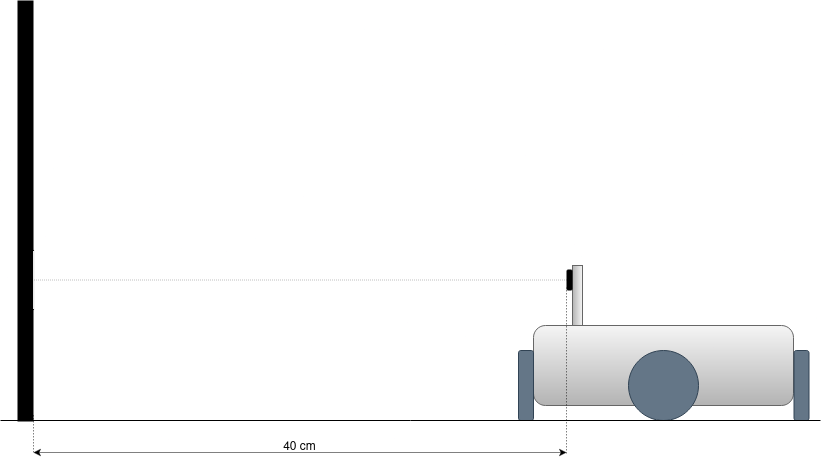
\includegraphics[width=1.0\linewidth]{images/robot_medicion_qr.png}
   \caption{Experiencia para la obtención de parámetros de calibración de la cámara}
   \label{fig:robot_medicion_qr}
\end{figure}

\subsection{Estimación de la posición del robot}

A partir de la lectura del código QR, obtenemos una estimación precisa de la posición del robot. Si el QR aparece centrado en la imagen, asumimos una alineación perfecta; de lo contrario, el desplazamiento del código en el eje horizontal lo interpretamos como una desviación en la ubicación del robot. Además, si el código se detecta con mayor tamaño, el robot se encuentra más próximo a él.

Cómo se mencionó anteriormente, el contenido del $payload$ incluye las coordenadas en donde se encuentra el código dentro del plano. Empleando el ejemplo donde un robot posicionado en la coordenada $(4,2)$ desea llegar a la coordenada $(4,0)$ donde se encuentra ubicado un código QR con las coordenadas descritas.

Cuando el robot se aproxima a su destino, la coordenada $(4,0)$, y se encuentra dentro del rango de distancia de reconocimiento de códigos QR, va a calcular la distancia tanto en el eje vertical como en horizontal y sumarla al payload del código QR para después poder reportar esa coordenada. Entonces en ese momento, así como muestra la figura \ref{fig:robot_posicion_1} el robot en realidad se encuentra ubicado en la coordenada $(4.2,0.5)$ y no en el centro de la celda como uno supone cuando no tiene el reporte de su ubicación en todo momento.

\begin{figure}[htpb]
   \centering
   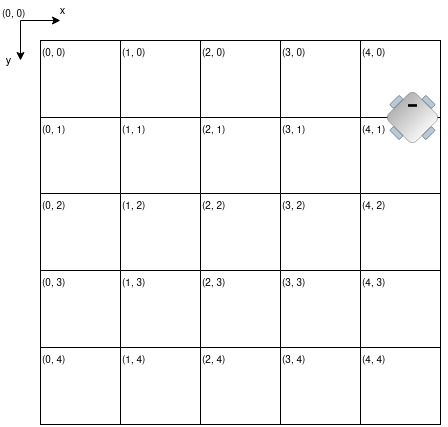
\includegraphics[width=0.9\linewidth]{images/robot_posicion_1.jpg}
   \caption{Robot posicionado en la coordenada $(4.2,0.5)$}
   \label{fig:robot_posicion_1}
\end{figure}

La captura de imágenes por parte del robot en movimiento queda representada en la figura \ref{fig:qrcamararobot} donde observamos una fotografía nítida y con buen enfoque, lo que permite un procesamiento de imágenes preciso.

\begin{figure}[htpb]
   \centering
   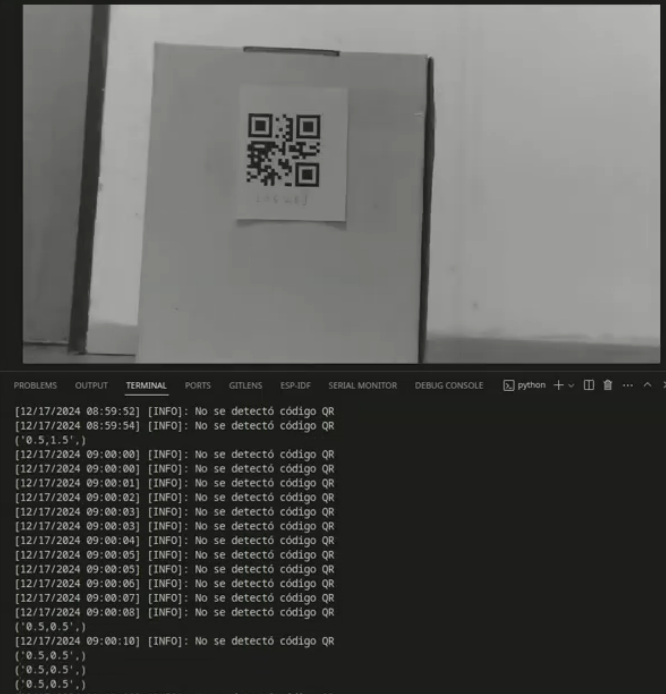
\includegraphics[width=0.9\linewidth]{images/qr.png}
   \caption{Imagen obtenida por el robot en movimiento en donde identifica un código QR, procesa el contenido del payload y lo envía por MQTT}
   \label{fig:qrcamararobot}
\end{figure}